\section{Palabras candidatas} % (fold)
\label{palabras_candidatas}
Para buscar las palabras candidatas a tener contrastes significativos en cuanto a la cantidad de ocurrencias en distintas provincias, elegimos el conjunto de las primeras 
cinco mil (5000) palabras con valor de la información más altas. El número 5000 surgió de ver la distribución de los valores de la información. Cómo se puede ver en 
el gráfico \ref{fig:ivalue} hay una caída pronunciada de la métrica y a partir de la palabra cuya posición es 4000 se ve que empieza a estabilizarse y los valores son 
muy cercanos a 0. Es por esto que nos pareció razonable dar un margen de 5000 palabras para evaluar manualmente las palabras del listado y, entre estas, seleccionar las palabras con contrastes significativos que tienen interés a nivel lingüístico.

Como era de esperar los topónimos como los nombres de ciudades y provincias son palabras que ocurren mayormente en sus respectivas regiones. Esto causa que haya gran variación en 
la cantidad de ocurrencias en las distintas provincias, lo que genera un valor alto en la métrica de valor de la información. Para detectar las palabras que tienen 
mayor interés lingüístico buscamos un conjunto de datos con los nombres de las localidades y departamentos de la República Argentina de modo tal que podamos resaltar para que el equipo de filólogos tenga una primera alerta sobre posible toponimia.

% Agregar algún comentario sobre regiones dialectales conocidas


\subsection{Regiones de palabras} % (fold)
\label{sub:regiones_de_palabras}

Una vez que calculamos las regiones que cubren un umbral para cada palabra, nos propusimos analizar cuales son las más frecuentes. Para eso generamos una lista con los conjuntos de provincias cuya cantidad sea menor a 7 y los ordenamos según su frecuencia. En la tabla \ref{tab:regiones} se muestran los primeros conjuntos de provincias obtenidos a partir de las primeras 5000 palabras con mayores contrastes de acuerdo al valor de la información.

\begin{table}
\centering

\begin{tabular}{|c|c|}
\hline
Conjunto de provincias                                 & Cantidad de Palabras  \\ \hline
Jujuy - Salta                                          & 24          \\
Mendoza - San Juan                                    & 19          \\
Neuquén - Río Negro                                   & 18          \\
Corrientes - Misiones                                 & 16          \\
Chaco - Corrientes - Formosa                           & 16          \\
Chaco - Corrientes                                    & 16          \\
Chubut - Santa Cruz                                   & 13          \\
Catamarca - La Rioja                                  & 12          \\
Santa Cruz - Tierra del Fuego                         & 12          \\
Corrientes - Entre Ríos - Formosa - La Rioja - Misiones  & 12          \\  %La Rioja está de más
Formosa - Misiones                                    & 12          \\
Corrientes - Formosa - Misiones                        & 12          \\
Córdoba - La Rioja                                    & 11          \\
Catamarca - Salta - Santiago del Estero - Tucumán       & 11          \\
Catamarca - Jujuy - La Rioja - Salta - Santiago del Estero - Tucumán & 10          \\
Chaco - Corrientes - Misiones                          & 10          \\
Chaco - Corrientes - Formosa - Misiones                 & 9           \\
Catamarca - Santiago del Estero - Tucumán              & 9           \\
Catamarca - Tucumán                                   & 9           \\
Salta - Tucumán                                       & 8           \\
Catamarca - Jujuy - Salta - Santiago del Estero - Tucumán& 8           \\
Neuquén - San Juan                                    & 7           \\ %no son contiguas pero están cercanas
Chubut - Santa Cruz - Tierra del Fuego                 & 7           \\
Buenos Aires - La Pampa                                & 7           \\
Salta - Santiago del Estero - Tucumán                  & 7           \\
Buenos Aires - La Pampa - Río Negro                     & 6           \\
Corrientes - Formosa                                  & 6           \\
Catamarca - Jujuy - Salta - Tucumán                     & 6           \\
Chaco - Corrientes - Entre Ríos - Formosa - Misiones     & 6           \\
Catamarca - Santiago del Estero                       & 6           \\
\hline
\end{tabular}
\caption{Indica cuantas palabras tienen un cubrimiento del 80\% de sus ocurrencias en cada conjunto de provincias a partir de las 5000 palabras con mayor contrastes (de acuerdo al valor de la información). Se suprimieron las regiones compuestas por una sola una provincia.}
\label{tab:regiones}
\end{table}

Mostramos algunos de los conjuntos de palabras de cada región en la tabla \ref{tab:palabrasRegiones} (ver apéndice). Sobre esta, podemos destacar que la mayoría de las regiones son compuestas por provincias contiguas.


\section{Problemas en el conjunto de datos}
\label{problemas_datos}

Cuando vimos las palabras con mayor valor de la información, nos dimos cuenta de que algunas palabras de la provincia de La Rioja eran provenientes de España. Analizando la causa de este ruido, nos dimos cuenta que la API de Twitter no realiza las búsquedas localizadas como uno esperaría. En particular, no solo se fija en los tuits geolocalizados, sino que también hace una búsqueda inversa a través de los nombres de las ciudades que tienen esa coordenada. Específicamente La Rioja es una provincia Argentina, como así también una provincia de España. Es por eso que al hacer búsquedas con las coordenadas de ciudades de La Rioja en Argentina, tuvimos resultados de tuits de España. Lo mismo sucedió con San Juan (capital de Puerto Rico), Santiago Del Estero (Santiago de Chile) y Córdoba (ciudad de Andalucía, España). A pesar de que los tuits no fueron escritos en Argentina, consideramos que su cantidad no es lo suficientemente grande como para tener resultados incorrectos.

% Histograma de la distribucion del valor de la información

\section{Caracterización de las palabras identificadas como contrastivas}
\label{caracterizacion_resultados}

Dentro de las palabras contrastivas identificadas a través de la métrica, podemos hacer una caracterización de ellas según el fenómeno lingüístico representan.

%A continuación presentamos en detalle cada fenómeno lingüístico y ejemplificamos con las palabras encontradas:

En base al listado de palabras identificados como contrastivas a partir de la métrica, se realizó una validación lingüística por lexicógrafos de la Academia Argentina de Letras. En esta, se realizó un estudio pormenorizado, palabra por palabra, en el cual los criterios seguidos para que una palabra sea relevante privilegiaron las posibilidades de que aquella forme parte del repertorio léxico de una comunidad de hablantes. Esto excluyó, como es tradicional en lingüística, nombres propios y topónimos locales, que la métrica sube a los puestos altos de las listas porque efectivamente su uso es abundante y contrastivo. 

En la lista \ref{it:caracterizacionLinguistica} presentamos una caracterización de las palabras La siguiente es una lista muy parcial, en la que hay apenas algunos ejemplos en cada categoría. Sin embargo sirve para ilustrar ejemplos de uso en el habla cotidiana de las palabras contrastivas identificadas. La lista completa arroja un resultado dentro del rango de las 300 palabras dignas de estudio por cada 5000 palabras, es decir, 1 palabra cada 17 aproximadamente. A pesar de que no existen otros proyectos que provean un término de comparación para evaluar el grado de éxito implicado en esta relación, no cabe ninguna duda de que, al menos en la detección de coloquialismos locales actualmente en uso, la herramienta plantea un verdadero punto de inflexión para la lexicografía contrastiva. Esta área del léxico es justamente la más elusiva, puesto que su impacto en cualquier medio impreso llega notablemente más tarde y, todavía más importante, en la mayoría de los casos no llega nunca. Se incluyeron como relevantes palabras que ya están incluidas en el Diccionario del habla de los argentinos \cite{academia2008diccionario}, dado que ese hecho es una confirmación adicional de la pertinencia de la ubicación que asignó la métrica.

Las formas cuyo uso se ejemplifica son las que están en negrita y solo en ellas se normalizó la tildación.

\begin{itemize}
  
  \label{it:caracterizacionLinguistica}
  
  \item \textbf{Coloquialismos o vulgarismos}

    \blockquote[Córdoba]{Perdon pero tenes que ser muy \textbf{culiado/a} para ir a mc y pedirte una ensalada}


    \blockquote[Mendoza]{Q \textbf{chombi} hacer un chiste y q la otra persona no se ría o no lo entienda}

    \blockquote[Neuquén]{Que \textbf{carnasas} poniendole rosas rojas a toda la ropa, para mi queda horrible sorry}

\item Indigenismos

    \blockquote[Formosa]{Te regalo ser \textbf{mitaí} y ir a jurar la bandera con el guardapolvo caliente ese y la corbata que te ahorca todo (Del guaraní mitaí “pequeño”)}

    \blockquote[Corrientes]{\textbf{Angá} mi negrito, esta triste (Del guaraní angá aprox. “pobre”) (Corrientes)}

    \blockquote[Tucumán]{Gracias tormenta \textbf{ura} por sonar como una pochoclera de chasquibums a las 3 de la mañana en mi ventana durante 50 minutos. (Valor despectivo. Del quechua ura “vulva, vagina”) }

\item \textbf{Gentilicios}

  \textbf{Casildense} (de Casilda), \textbf{concordiense} (de Concordia) y \textbf{obereño} (de Oberá).

\item \textbf{Voces no marcadas en registro, que aluden a una realidad local}

  \blockquote[San Juan]{Quiero a alguien que me diga vamos a comer \textbf{piadinas}, un pancho, un chori, una hamburguesa lo que sea y soy feliz}

  \blockquote[Misiones]{\textbf{Tareferos} que reclamaban asistencia interzafra en Posadas estarían preparando una protesta para hoy en la Fiesta del Inmigrante en Oberá.}

  \blockquote[Jujuy]{Me encantan los bohemios anti sistema que usan vans. Es como que seas ecologista y uses un cuaderno hecho con media \textbf{yunga}.}

\item \textbf{Voces sinónimas de otras más usuales en Buenos Aires}

  \blockquote[Chaco]{Teres, \textbf{pororós} y pelis con Carlita y Flor}

  \blockquote[San Juan]{Ver un negro \textbf{chuño} con musculosa y gorro.. se ve que el tipo no quería pasar ni frío ni calor.}

  \blockquote[Formosa]{Tenía la re expectativa para este sábado y al final \textbf{trancó} todo }

\item \textbf{Leísmo}

  \blockquote[Misiones]{No te olvides de \textbf{saludarle} a tu suegro hoy}

  \blockquote[Misiones]{Vine a \textbf{visitarle} a mis primas y estan re colgadas, para eso me quedaba en mi casa no maaa }

  \blockquote[Formosa]{A \textbf{esperarle} a nahuel, que traiga los teresss }

\item \textbf{Fusiones y acrónimos que pueden señalar pronunciación o alta frecuencia de uso}

  \blockquote[Buenos Aires]{Los sueños de la siesta me dejan \textbf{patra} }

  \blockquote[Córdoba]{Si mañana me dice q no, voy sola, necesito ver esa pelicula en el cine siosi}

\item \textbf{Voces consideradas generales pero que, al aparecer en la lista, permitieron verificar su contrastividad en frecuencia de uso al menos con respecto a España}

Ejemplos: \textbf{pavada}, \textbf{distrital} y \textbf{cariño}.

\item \textbf{Voces sospechadas generales pero con acepción local diferente}

  \blockquote[Mendoza]{Mañana que alguien \textbf{atine} con parque y porrones}

  \blockquote[San Juan]{\textbf{Mansas} ganas de sentarme a tomar un te con semitas}

  \blockquote[Tierra del Fuego]{\textbf{Habilítenme} una nueva espaldaa}

  \blockquote[San Juan]{sigo \textbf{asada} por cosas que han pasado hace como dos dias, que falla (Mendoza) / Que \textbf{asada} estoy, tengo la cabeza echa un lío}


\item \textbf{Voces con una morfología propia de una región}

Ejemplo: terminación aso/asa con base adjetiva.

  \blockquote[San Juan]{Creo que va a estar \textbf{malaso} lo de esta noche } 

  \blockquote[San Luis]{estoy subiendo un mix re \textbf{chomaso} que hice anoche }

  \blockquote[Córdoba]{Esta \textbf{locasa} esa mina para hacer eso}

\item \textbf{Formas indicadoras de pronunciación usual}

  \blockquote[Tucumán]{Menos mal que soy de los chetos de la carne y mañana tengo \textbf{asao} todo el dia jajajajaj}

  \blockquote[Catamarca]{Un lunes con buen humor ta \textbf{pasao} }

  \blockquote[Corrientes]{Ahora a la mañana tengo q ir hacerme la tarjebus jajajajj \textbf{mavale} q me estoy por levantarrr jajajaj}

\item \textbf{Formas verbales coloquiales con sustantivos o adjetivos como base}

  \blockquote[Neuquén]{Me calma mucho \textbf{mimosear} a mi perro }

  \blockquote[Buenos Aires]{Me vine a acostar y ya me dicen que parezco de 80 años ME CHUPA UN HUEVO LO QUE PIENSEN, DEJENME \textbf{ABUELEAR} }

  \blockquote[Tierra del Fuego]{Estaría bueno que ari venga aunque sea a saludarme y que no se quede todo el tiempo \textbf{pollereando}.}

\item \textbf{Variantes ortográficas, operativas para incorporarlas algunas como tales y también para verificar la alta frecuencia de uso}

Ejemplos: culiado (adj. despect. o fórmula de tratamiento de confianza) y tereré.

  \blockquote[Córdoba]{Q paja volver al colegio \textbf{culiaa}}

  \blockquote[Córdoba]{Que pajero el \textbf{qliao} este.}

  \blockquote[Córdoba]{Quiero recitaaal \textbf{qliaaaa}}

  \blockquote[Entre Ríos]{\textbf{Tereresss} y pile con todos mis primisss}

  \blockquote[Corrientes]{No se si hacerme un \textbf{tere} o un mate para pasar la siesta}

  \blockquote[Chaco]{Es lo mas lindo no ir al colegio y quedarme a tomar \textbf{teresss}}


\item \textbf{Vesres} : Creación de palabras por inversión de sílabas que se usa jergalmente o con fines humorísticos.

  \blockquote[Corrientes]{Estoy en lo de villa mateando con él y jimmy. Pinta \textbf{sogui} abundante más tarde dijeron }

  \blockquote[Chaco]{Uhhh me acuerdo si no habré saltado el muro del aguapey par colarme a los \textbf{cequin}. (cequín “fiesta de quince”)}

\item \textbf{Intejercciones}

  \blockquote[Formosa]{\textbf{Aijué}, encima me decís vieja, re que no pinta esto facundo jaja ya te dije como es la onda, fin }

  \blockquote[Formosa]{\textbf{Ains}, una mujer hablando de fútbol.}

  \blockquote[Corrientes]{Al fin una buena: hora libreeee! \textbf{Yirr} }

\item \textbf{Guaranismos}
\label{sub:guaranismos}
Cabe destacar la detección de términos en guaraní en la región  guaranítica\footnote{Teniendo a las regiones dialectales marcadas por Vidal de Battini}.
Un ejemplo de esto fueron las palabras \textit{angá}, \textit{angaú} y \textit{mitaí}.  Si bien estas palabras provienen del guaraní, son utilizadas en oraciones en español.
Como se puede ver en la tabla \ref{tab:guaranismos} el contraste entre las frecuencia normalizadas \footnote{La frecuencia normalizada es una medida de estandarización que indica la cantidad de veces que aparece una determinada forma por cada millón de palabras.} de la región guaranítica y la del litoral da una noción de la importancia que tienen estos términos en norte argentino. 


\end{itemize}





\begin{table}
\centering

\begin{tabular}{|l|cc|cc|}
\hline
 & \multicolumn{2}{c}{Región Guaranítica} & \multicolumn{2}{c}{Región Litoral} \\ \hline
      & \#Ocurrencias & Frecuencia Normalizada & \#Ocurrencias & Frecuencia Normalizada \\
Angá  & 548              & 45,03       & 6             & 0,21                  \\
Angaú & 205               & 16,84   & 0               & 0                     \\
Mitai & 175              & 15,69      & 1              & 0,036    \\ \hline              
\end{tabular}

\caption{Cantidad de ocurrencias y frecuencias normalizadas de las palabras en la región guaranítica y la del litoral. La cantidad total de palabras en la región guaranítica es de 12.167.635, mientras que la cantidad de términos en la región litoral es 27.477.861 }
\label{tab:guaranismos}
\end{table}

Estos términos serán agregados al diccionario del habla de los argentinos \cite{academia2008diccionario}.


\section{Test Hipergeométrico}
Luego de realizar el listado de palabras ordenado por el valor de la información se aplicó un test estadístico para tener mayor confianza de que las palabras clasificadas como contrastivas realmente tienen esta propiedad y no fueron producto del azar. Se seleccionó un conjunto de palabras significativas a nivel lingüístico a partir de las 5000 palabras consideradas más contrastivas por nuestra métrica. 

Decidimos elegir el test hipergeométrico ya que queremos ver que la palabra sobre la que se hace el test no estuvo sobrerrepresentada en comparación con la población. Asumimos que la cantidad de ocurrencias de una palabra se puede modelar con una distribución hipergeométrica ya que se puede pensar como un experimento donde se obtuvieron $k$ palabras exitosas en una región con $n$ palabras y un total de $N$ palabras en la Argentina. Las regiones que utilizamos para cada palabra son el conjunto de provincias que cubren el 80\% de las ocurrencias de dicho término. Luego, queremos calcular la significancia estadística de haber obtenido esas $k$ palabras exitosas.

Luego, por cada palabra seleccionada como contrastiva le aplicamos el test estadístico con la siguiente hipótesis nula: la palabra tienen un uso homogéneo en las distintas regiones de la Argentina, es decir que la frecuencia de ocurrencias de cada palabra debería ser similar independientemente de la región.
Por lo tanto, en caso de que la palabra sea contrastiva deberíamos obtener una baja probabilidad de haber obtenido diferencias entre las frecuencias de la palabra en una región con el resto del país.  
% que la cantidad de ocurrencias de la palabra en la región elegida es mayor a lo observado. 
Por lo tanto, sea  cantPalabrasW(Region) igual a la cantidad de ocurrencias observada de la palabra en la región a analizar.


\begin{table}[ht]
\centering
\label{tab:contingencia}
\begin{tabular}{lccc}
\hline
& \#Palabras Sobre Region &\#Palabras en el resto de Argentina &Total \\ \hline
\# Palabras w &   k & K-k & K \\ 
\# Palabras $\neq$ w & n-k & N + k - n - K  & N - K \\ 
Total & n & N -n & N \\ \hline
\end{tabular}
\caption{Tabla de contingencia}

\end{table}



$$
\begin{cases}
H_0 :  x > cantPalabrasW(Region) \\
H_1 : x \leq cantPalabrasW(Region)
\end{cases}
$$  
siendo x la esperanza de la variable aleatoria que representa la cantidad de palabras exitosas en esa región.

% agregar gráficos de palabras comunes, con los parametros de la distribucion
% hacer un grafico de la distribución estimada (y la observada) de la cantidad de ocurrencias de la palabra 
En primer lugar hicimos el test estadístico sobre las palabras del conjunto de datos de desarrollo para ver resultados preliminares. El test lo realizamos sobre palabras candidatas a ser contrastivas informadas por nuestra métrica. Una vez realizado este test obtuvimos los p-valores de la figura \ref{fig:p-valores}. Debido a que realizamos múltiples test tuvimos que aplicarle una corrección para evitar falsos positivos. Decidimos utilizar la corrección de Benjamini–Hochberg.
 % Hablar sobre test multiples y correcciones posibles 


\begin{figure}[!ht]\centering
    \includegraphics[width=\linewidth]{./images/pvalores.png}
    \caption{Gráfico de dispersión de los p-valores del test hipergeométrico sobre las primeras 5000 palabras} 
    \label{fig:p-valores}   
\end{figure}


Ante los p-valores tan bajos, decidimos hacer el test estadístico sobre palabras que consideramos que no tendrían porque tener una frecuencia muy distinta en las distintas regiones. Realizamos el test para las palabras \{que, cuando, hola\} y estos también dieron p-valores menores a 0.001. Frente a esta situación investigamos las posibles causas de este fenómeno.


Un estudio de Adam Kilgariff titulado \textit{Language is never, ever, ever, random}\cite {kilgarriff2005language} comenta que debido el lenguaje no es aleatorio realizar test estadísticos ... llega a conclusiones que no aportan nada de información ya que la premisa del test estadístico es falsa. Por lo tanto, al ser falsa la premisa uno obtiene una implicación, en nuestro caso el resultado del test, trivialmente verdadera. 
% Hacer el grafico dependiendo de las frecuencias
% Comentar acerca del experimento en el que ve que para las palabras con mas frecuencia hay un mayor error. esto quizas explica porque las palabras con menos valor de la informacion tienen p-valores mas altos 
Kilgariff también hace un análisis sobre trabajos previos y comenta el caso en el que un estudio quería encontrar palabras con frecuencias significativas entre el inglés británico y el americano, representados por el Corpus Brown(inglés americano) y el Lancaster-Oslo-Bergen Corpus(inglés británico). Para cada palabra testearon la hipótesis nula la cual afirmaba que la diferencia entre las frecuencias sobre los dos corpus se debía a una fluctuación  aleatoria. El test lo hicieron a partir de muestras obtenidas aleatoriamente de los corpus mencionados. En este estudio se marcaron las palabras donde la hipótesis nula se rechazaba con distintos niveles de confianza. Las listas sugieren que la mayor parte de las palabras \textit{comunes} fueron marcadas, es decir que el test estadístico sugería que todas estas palabras tenían diferencias significativas en su uso. Esto que comenta Kilgariff es lo que tuvimos como resultado a partir de nuestro test hipergeométrico. Lo interesante es que el autor atribuye ese fenómeno a la esencia no aleatoria del lenguaje.Si bien sabíamos que al realizar el test hipergeométrico asumíamos que la probabilidad de que ocurra una palabra era independiente, pensamos que esta suposición no iba a afectar tanto los resultados como lo hizo.

Un estudio más reciente, Lijffijt et al. \cite{lijffijtsignificance} propone ciertas alternativas para hacer un test de hipótesis en los cuales no se asume el modelo de \textit{bag-of-words}. En ese trabajo se analizaron el test t de Welch, el test de los rangos con signo de Wilcoxon(Wilcoxon rank sum), el de Bootrstrap y el de tiempo entre llegadas (inter-arrival time). Lijffijt explica que \blockquote[lijffijtsignificance]{la diferencia entre estos tests con los que asumen el modelo de \textit{bag-of-words}( ${\chi}^2$ y log-likelihood test) reside en la representación de los datos, ergo la unidad de observación:
Para los tests que suponen los modelos \textit{bag-of-words}, los datos se representan en una tabla de contingencia de 2x2 y el número de muestras equivale al número de palabras en el corpus, mientras que en los otros cuatro tests, los datos son representados en una lista de frecuencias o una lista de \textit{tiempos de llegada}. En estos casos, el número de muestras es mucho menor que la cantidad de palabras en el corpus(...) El número de muestras generalmente determina nuestro nivel de seguridad en relación a los valores estimados, y los resultados expermientales muestran que los tests de modelos de \textit{bag-of-words} tienen una excesiva alta confianza en los valores estimados de la frecuencia media de las palabras, en el contexto de comparación estadística entre dos corpus}

% Hablar sobre las alternativas que propone Lijffijt
%TODO: agregar los resultados de las palabras del test hipergeometrico.
% las palabras raras, y el grafico de pvalores. a partir de eso comentar el trabajo de kilgariff 
% que habla de test de hipotesis, el error de asumir que las palabras vienen de un proceso aleatorio.

\section{Test t de Welch}
Basándonos en las propuestas de Lijffijt, decidimos utilizar el test de Welch. Este nos provee un valor de probabilidad para rechazar la hipótesis nula la cual afirma que las medias de las dos distribuciones son iguales. Sean $S$ y $T$ dos corpus y sea $q$ la palabra sobre la cual se va a hacer el test, sea $x_1$ la media de la frecuencia de la palabra $q$ sobre los textos de $S$, y sea $s_1$ la desviación estandar. Análogamente, sea $x_2$ la media de la frecuencia de $q$ en los textos $T$ y $s_2$ la desviación estandar. El estadístico $t$ se calcula con la ecuación \ref{eq:estadistico_welch}. Las asunciones del test consisten en que todos los textos son estadísticamente independientes y que la media de las frecuencias proviene de una distribución normal. En nuestro caso, agrupamos todos los tuits de cada usuario representando un texto. De esta manera, cada provincia tiene alrededor de 900 textos formados por distintos usuarios \footnote{La cantidad de usuarios recolectados por cada provincia se encuentra detallada en la tabla \ref{tab:cantidades}}. Luego, el test es aplicado a cada palabra con las frecuencias entre dos corpus: uno está formado por todos los textos de los usuarios que provienen de las provincias en donde se cubre el 80\% de las ocurrencias, el otro consiste en los textos creados por usuarios del resto de las provincias.

\begin{equation}
\label{eq:estadistico_welch}
 t = \frac{x_1-x_2}{\sqrt{\frac{s_1^2}{\lvert S \rvert}+\frac{s_2^2}{\lvert T \rvert}}}  
\end{equation}

Calculamos la taza de rechazo para las palabras en distintos intervalos del listado ordenado según las tres métricas elegidas: la métrica que tiene en cuenta la entropía de palabras, la valora la entropía de personas, y la que contiene a los dos factores.En la figura \ref{fig:rechazo_metricas} se muestran los resultados. La métrica elegida, la cual tiene a ambos factores en consideración tiene una mejor taza de rechazo de la hipótesis nula en las palabras consideradas contrastivas y una menor taza de rechazo para el resto. 
Es importante notar que el test de Welch que realizamos tiene como muestras las distintas frecuencias de todos los usuarios en cada región. Por lo tanto es razonable obtener un resultado como este, en el cual las métricas que consideran la dispersión de las frecuencias sobre todos los usuarios para distinguir el nivel de contrastividad de la palabra.

\begin{figure}[!ht]\centering
  
    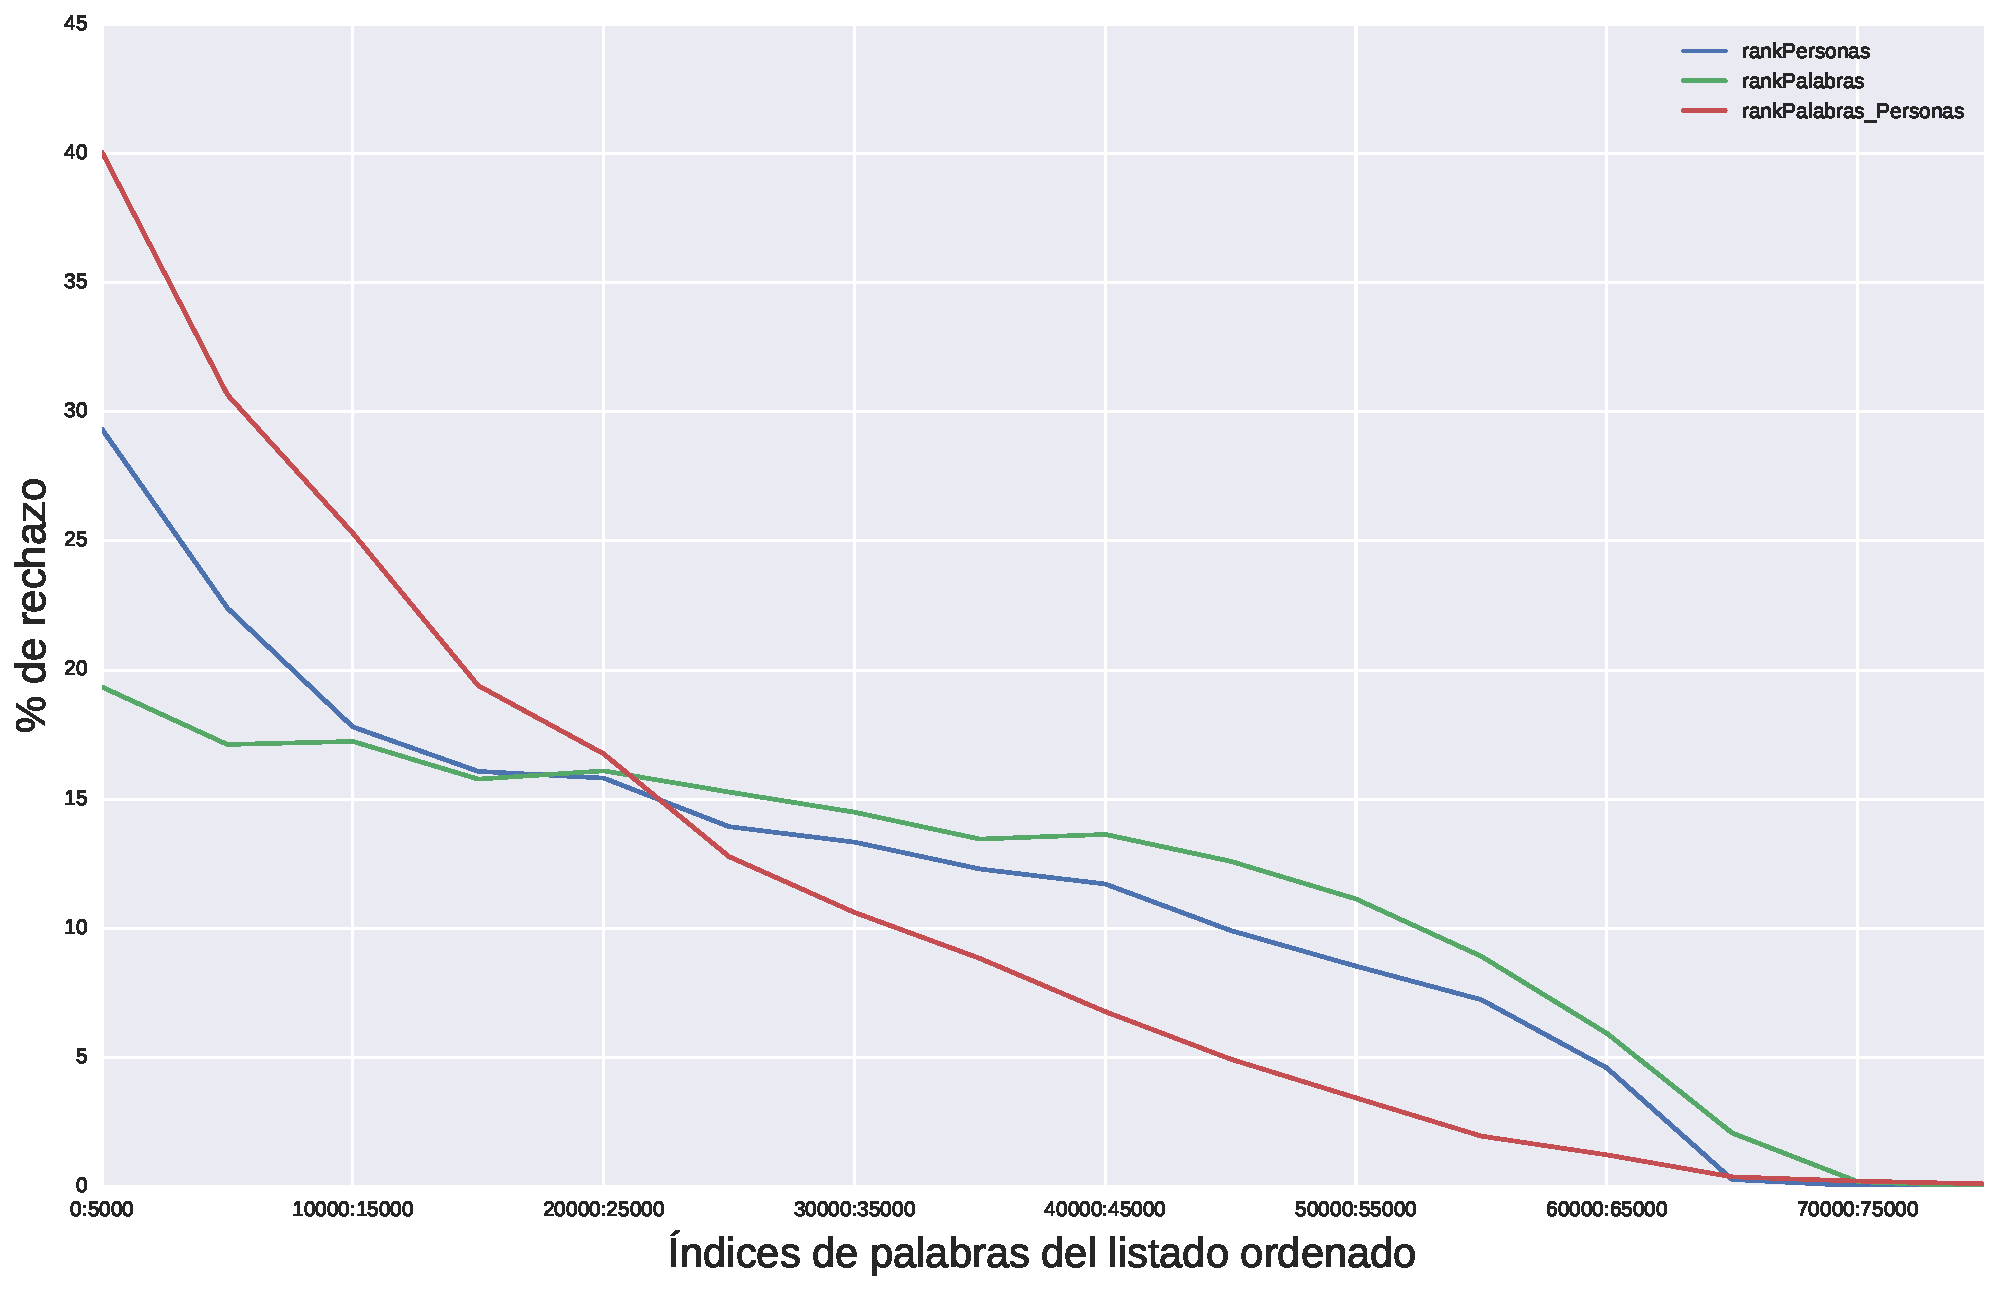
\includegraphics[width=\linewidth]{./images/rechazo_metricas.pdf}
    \caption{Resume la tasa de rechazo de la hipótesis nula en los distintos conjuntos de palabras, los cuales varían según el índice de estas en el listado ordenado según la métrica elegida.} 
    \label{fig:rechazo_metricas} 

\end{figure}

También es importante destacar que a medida que uno se aleja de las palabras más contrastivas de acuerdo a nuestra métrica, la tasa de rechaza es menor. Esto refleja el buen comportamiento de la métrica. Este resultado se puede observar también en la figura \ref{fig:pvalores_sinBonferroni} donde se detalla la distribución de los p-valores en el conjunto de las primeras 5000 palabras y el resto de los términos del listado.

\begin{figure}[!ht]\centering
  
    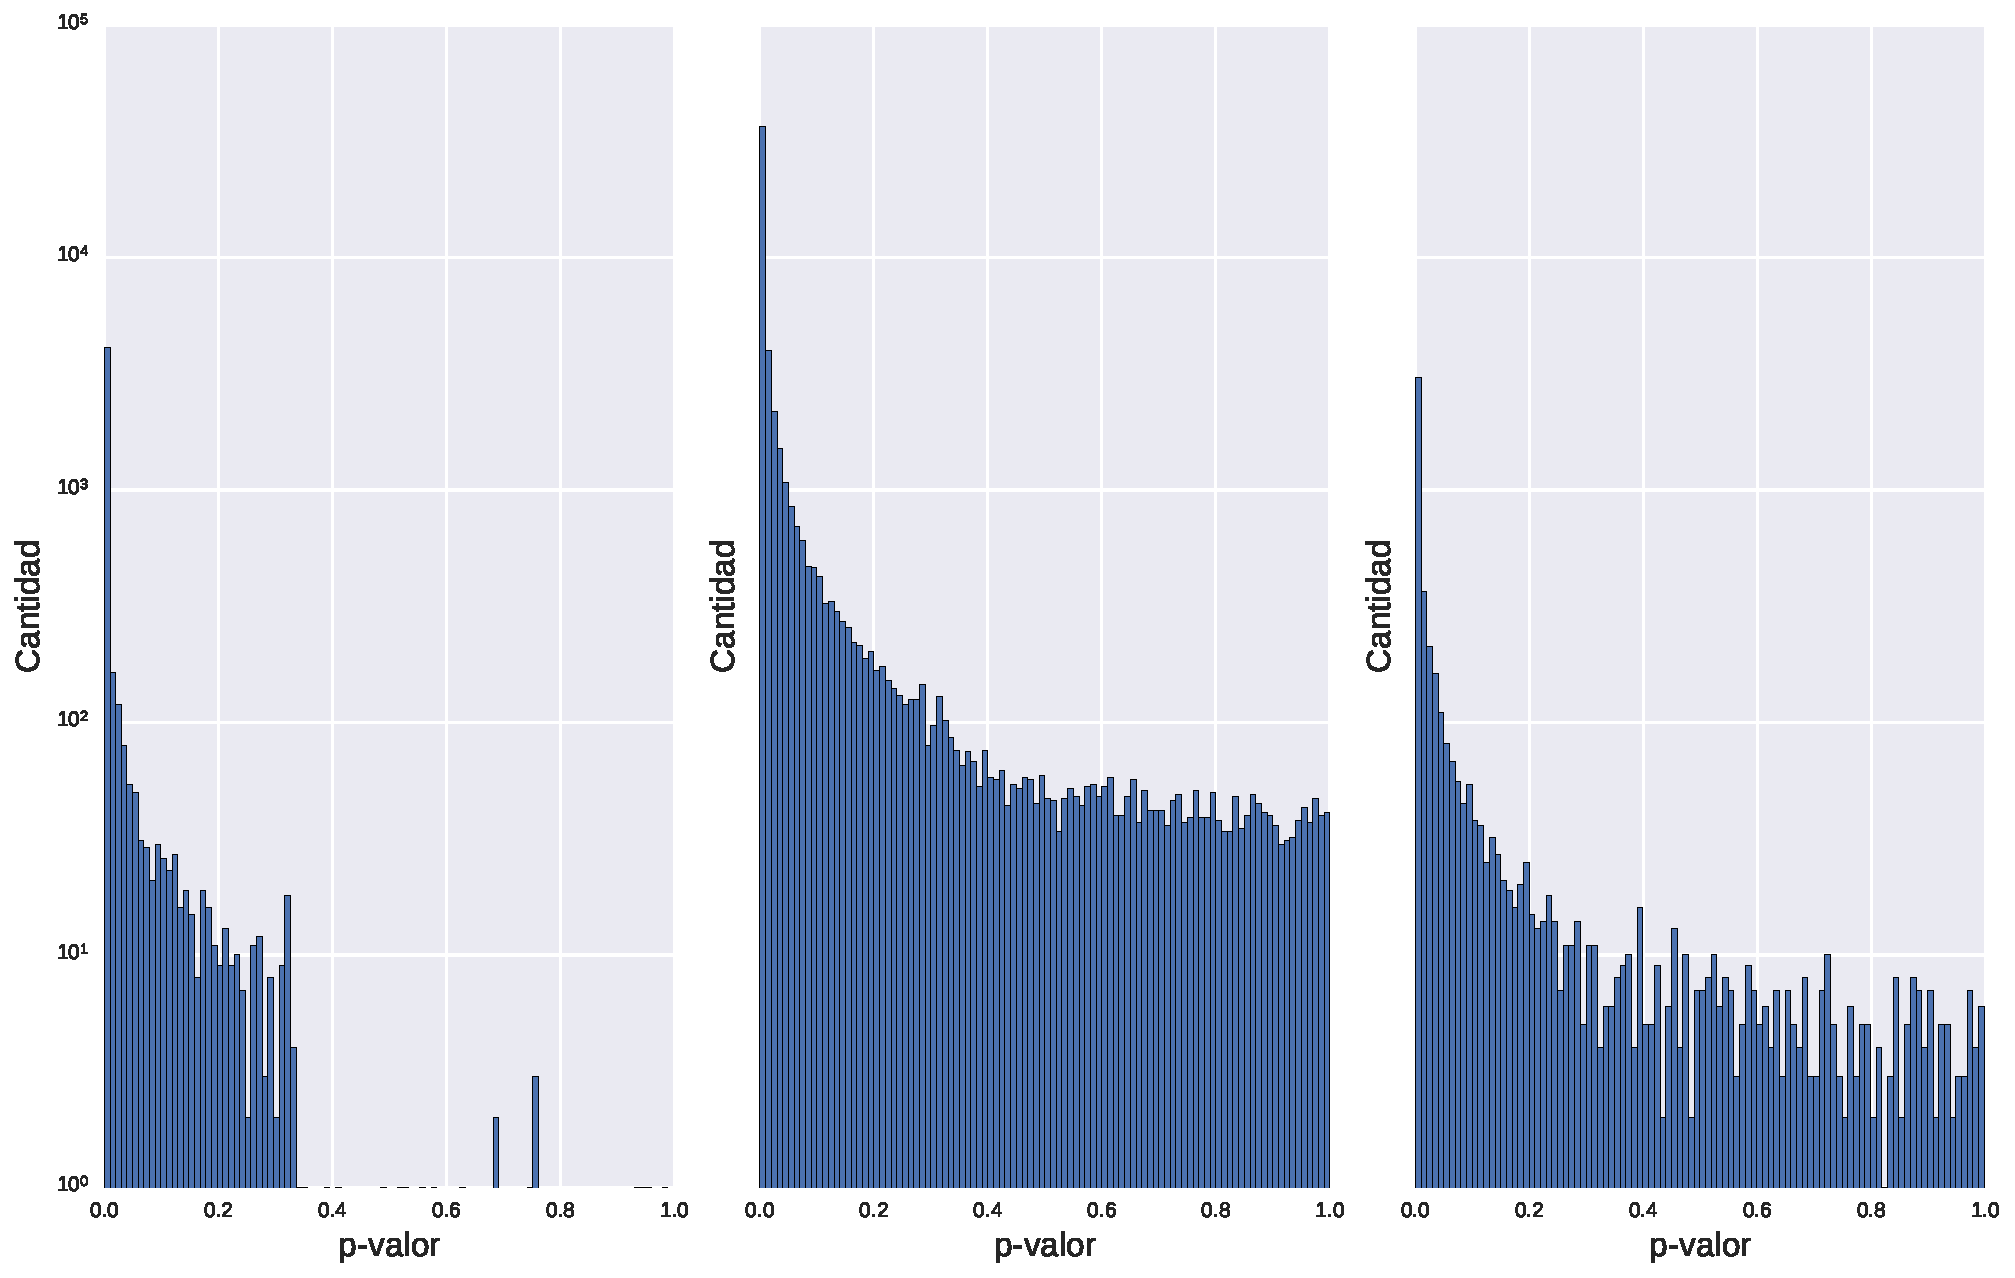
\includegraphics[width=\linewidth]{./images/pvalores_sinBonferroni.pdf}
    \caption{Distribución de p-valores (sin corrección de tests múltiples) en las primeras 5000 palabras del listado y el resto de las palabras.} 
    \label{fig:pvalores_sinBonferroni} 

\end{figure}

